% $HeadURL: https://sbgn.svn.sourceforge.net/svnroot/sbgn/trunk/documents/specifications/EntityRelationship/Level1/sources/unspecified.tex $

\color{red}

\subsection{Glyph: \glyph{Unspecified entity}}
\label{sec:unspecifiedEntity}

The simplest type of EN is the \glyph{unspecified entity}: one whose type is unknown or simply not relevant to the purposes of the model.  This arises, for example, when the existence of the entity has been inferred indirectly, or when the entity is merely a construct introduced for the needs of the model, without direct biological relevance.  These are examples of situations where the \emph{unspecified entity} glyph is appropriate.  (Conversely, for cases where the identity of the entities \emph{is} known, there exist other, more specific glyphs described elsewhere in the \SBGNERLone specification.)

\begin{glyphDescription}

\glyphSboTerm SBO:0000285 ! material entity of unknown nature 

\glyphContainer An \glyph{unspecified entity} is represented by an elliptic container, as shown in \fig{unspecified}.

\glyphLabel An \glyph{unspecified entity} is identified by a label placed in an unbordered box containing a string of characters.  The characters can be distributed on several lines to improve readability, although this is not mandatory.  The label box must be attached to the center of the container.  The label may spill outside of the container.

\end{glyphDescription}

\begin{figure}[H]
  \centering
  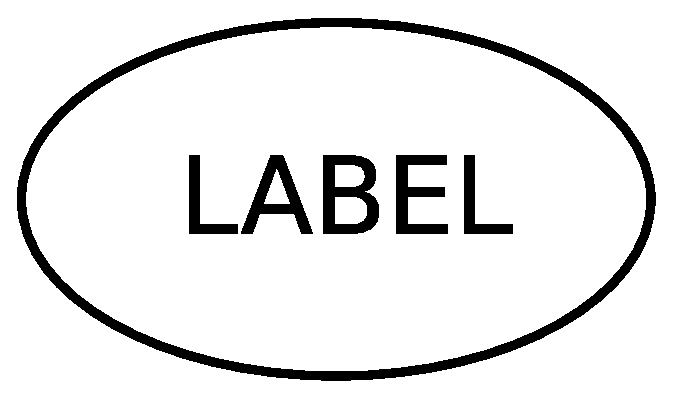
\includegraphics[scale = 0.3]{images/unspecified}
  \caption{The \ER glyph for \glyph{unspecified entity}.}
  \label{fig:unspecified}
\end{figure}

\normalcolor

% The following is for [X]Emacs users.   Please leave in place.
% Local Variables:
% TeX-master: "../sbgn_ER-level1"
% End:
